\PassOptionsToPackage{unicode}{hyperref}
\PassOptionsToPackage{naturalnames}{hyperref}
\documentclass[12pt, xetex, xcolor=pdftex, dvipsnames]{beamer}
\usetheme{metropolismyfont}
\usepackage{dcolumn} % for apsrtable outputs
\usepackage{xunicode} % extra support for unicode
\usepackage{xltxtra} % implements some odds-and-ends features
\usepackage{verbatim} % for multiple-line comments
% to fix a problem in line-breaks
% see "http://zrbabbler.hp.infoseek.co.jp/xelatex.html"
\XeTeXlinebreaklocale "ja"
\XeTeXlinebreakskip=0pt plus 1pt
\XeTeXlinebreakpenalty=0
\def\<{\@ifstar{\zx@hwback\nobreak}{\zx@hwback\relax}}
\def\zx@hwback#1{\leavevmode#1\hskip-.5em\relax}

\usepackage{color}
\usepackage{listings}
\lstset{%
    language={Python},%
    basicstyle={\footnotesize},%
    identifierstyle={\footnotesize},%
    commentstyle={\footnotesize\color{mLightGreen}},%
    keywordstyle={\footnotesize\color{mLightBrown}},%
    stringstyle={\footnotesize\color{mDarkBrown}},%
    frame={tblr}%
}

\usepackage{graphicx}

\AtBeginSection[]{
    \begin{frame}{目次}
        \setbeamertemplate{section in toc}[sections numbered]
        \tableofcontents[currentsection, hideallsubsections]
    \end{frame}
}

\title{引き継ぎ資料 Vol.5}
\subtitle{Pythonのライブラリ等}
\date{2016/09/??}
\author{}
\institute{}
\begin{document}
\maketitle
\begin{frame}{コンセプト}
    ``私はこんなライブラリ・ツールを使ってますよ''

    要は布教
\end{frame}
\begin{frame}{今さら説明しないやつ}
    \begin{description}
        \item[numpy] 数値計算
        \item[scipy] (numpyにはない)数値計算
        \item[matplotlib] グラフ作成
    \end{description}
\end{frame}
\begin{frame}{目次}
  \setbeamertemplate{section in toc}[sections numbered]
  \tableofcontents[hideallsubsections]
\end{frame}
\section{導入}
\begin{frame}
    Pythonには大体なんでもあるよ!
\end{frame}
\begin{frame}
    すでにあるライブラリを上手に使おう!
\end{frame}

\section{multiprocessing}
\begin{frame}{multiprocessing}
    作業者を増やして高速化

    \begin{figure}
        \centering
        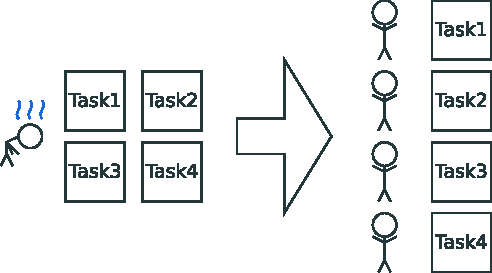
\includegraphics{img/multitask.pdf}
    \end{figure}
\end{frame}
{
    \setbeamertemplate{frame footer}{%
        Photo credit: \href{https://www.flickr.com/photos/hjmediastudios/7906332058/}{HJ Media Studios} %
        via \href{http://foter.com/}{Foter.com} %
        / \href{http://creativecommons.org/licenses/by-sa/2.0/}{CC BY-SA}%
    }
    \usebackgroundtemplate{
\includegraphics[width=\paperwidth]{img/clones.png}}
    \begin{frame}[b]
        \alert{\textbf{Q.}} Macのなかには作業者が何人?
        \pause
        \alert{\textbf{A.}} 8人{\tiny (環境によるが目安として)}
    \end{frame}
    \begin{frame}[b]
        8倍速で実行可能
    \end{frame}
}
\begin{frame}{いわゆるプログラミング用語}
    作業者を作る = スレッド(Thread)を立てる
\end{frame}
\begin{frame}{Pythonのスレッド}
    Pythonのスレッドは一人で幾つかの作業

    \begin{figure}
        \centering
        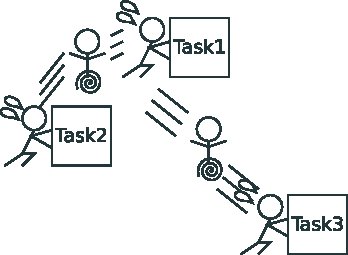
\includegraphics{img/python_thread.pdf}
    \end{figure}

    \pause
    いくつ立てても高速化はされない
\end{frame}
\begin{frame}{そこで登場!}
    multiprocessingはProcess操作を提供

    Process = 作業者
\end{frame}
\begin{frame}[fragile]{例}
    \lstinputlisting[firstline=2, lastline=14]{../src/example_multiprocessing.py}
\end{frame}
\begin{frame}{実行時間}
    約3倍の実行速度

    \begin{table}[b]
        \begin{tabular}{ll}\hline
            関数名 & 実行時間[秒] \\\hline
            single\_process & 6.62 \\\hline
            multi\_process & 2.02 \\\hline
        \end{tabular}
    \end{table}
\end{frame}
\begin{frame}{注意点}
    \begin{itemize}
        \item 5プロセスで実行しているが5倍にはならない
        \begin{itemize}
            \item プロセスの生成はそれなりに大変
        \end{itemize}
        \item なんでもかんでも別プロセスにしない!
        \begin{itemize}
            \item デバッグがし難い
            \item ここぞという時の切り札
        \end{itemize}
    \end{itemize}
\end{frame}

\section{docopt}
\begin{frame}{docopt}
    コマンドラインオプションを扱うライブラリ

    Python標準のargparseより簡単かつかっこいい
\end{frame}
\begin{frame}[fragile]{インストール方法}
    普通にpipで導入
    \begin{lstlisting}[language=Bash]
$ pip install docopt
    \end{lstlisting}
\end{frame}
\begin{frame}{docopt}
    \textbf{\alert{コメントから}}コマンドラインオプションを指定
\end{frame}
\begin{frame}[fragile]{例}
    \lstinputlisting{../src/example_docopt.py}
\end{frame}
\begin{frame}[fragile]{例}
    \lstinputlisting[firstline=3, lastline=5]{../src/example_docopt.py}

    実行
    \begin{lstlisting}[language=Bash]
$ python example_docopt.py hoge fuga
{'--arg1': False,
 '--ball': False,
 '-h': False,
 '<arg1>': 'hoge',
 '<arg2>': 'fuga'}
    \end{lstlisting}
\end{frame}
\begin{frame}[fragile]{例}
    \lstinputlisting[firstline=3, lastline=5]{../src/example_docopt.py}

    実行
    \begin{lstlisting}[language=Bash]
$ python example_docopt.py -a hoge fuga
{'--arg1': True,
'--ball': False,
'-h': False,
'<arg1>': 'hoge',
'<arg2>': 'fuga'}
    \end{lstlisting}
\end{frame}
\begin{frame}
    \begin{block}{Pros.}
        \begin{itemize}
            \item 書くのが楽
            \item コメントとプログラムが必ず一致
        \end{itemize}
    \end{block}
    \begin{block}{Cons.}
        \begin{itemize}
            \item 重い
            \item \url{http://docopt.org/}をよく見ないとたまに変な動作
        \end{itemize}
    \end{block}
\end{frame}
\begin{frame}{用途}
    ソースコードの中にファイル名とか入れるのやめよう

    ファイルの位置が変わったらソースも書き換え

    コマンドラインオプションにしておけば呼び出し時に自由自在
\end{frame}

\section{sphinx}
\begin{frame}{sphinx}
    Pythonに関するツール\footnote{sphinxはPython限定ではない}

    Anacondaにはデフォルトで搭載
\end{frame}
\begin{frame}{用途}
    \begin{enumerate}
        \item 一定の方式に則ってコメントを記述
        \item Sphinxで処理
        \item プログラムのドキュメント完成
    \end{enumerate}
\end{frame}
\begin{frame}{例: コメント記述}
    Sphinxでは決まったルールでコメントを書くことが必要

    \begin{block}{ルール}
        \begin{itemize}
            \item Sphinx形式(デフォルト)
            \item Google形式\\
                \url{http://www.sphinx-doc.org/en/stable/ext/example_google.html}
            \item NumPy形式\\
                \url{http://www.sphinx-doc.org/en/stable/ext/example_numpy.html}
        \end{itemize}
    \end{block}
\end{frame}
\begin{frame}[fragile]{例: コメント記述(Google形式)}
    \lstinputlisting[%
        basicstyle={\scriptsize},%
        commentstyle={\color{mLightGreen}},%
        keywordstyle={\color{mLightBrown}},%
        stringstyle={\color{mDarkBrown}},%
        lastline=16%
    ]{../src/example_sphinx/src/program.py}
\end{frame}
\begin{frame}[fragile]{例: Sphinxで処理}
    ソースコードからドキュメントの元を生成

    \begin{lstlisting}[language=Bash]
$ sphinx-apidoc -F -o doc src
    \end{lstlisting}

    srcの中身を元にdocにドキュメントの元を生成
\end{frame}
\begin{frame}{例: docフォルダの中身}
    \begin{description}
        \item[*.rst] ドキュメントの元
        \item[Makefile] ドキュメント生成のプログラム
        \item[conf.py] 設定が書かれたpythonファイル
    \end{description}
    \begin{figure}
        \centering
        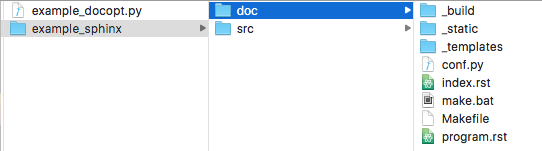
\includegraphics[width=8cm]{img/sphinx.png}
    \end{figure}
\end{frame}
\begin{frame}{例: conf.py}
    設定が書かれたpython形式のファイル

    \begin{block}{記述が必要な事項}
        \begin{itemize}
            \item extensionsに"sphinxcontrib.napoleon"追加\\
                Google形式コメントの有効化
            \item languageを"ja"に設定\\
                自動生成される部分を日本語化
            \item テーマの設定
        \end{itemize}
        詳細はサンプルコードを参照
    \end{block}
\end{frame}
\begin{frame}[fragile]{例: ドキュメント完成}
    ドキュメントディレクトリへ移動
    \begin{lstlisting}[language=Bash]
$ cd doc
    \end{lstlisting}

    htmlファイルの生成
    \begin{lstlisting}[language=Bash]
$ make html
    \end{lstlisting}

    pdfファイルの生成
    \begin{lstlisting}[language=Bash]
$ make latexpdfja
    \end{lstlisting}
\end{frame}
\begin{frame}{例:結果(html)}
    \begin{figure}
        \centering
        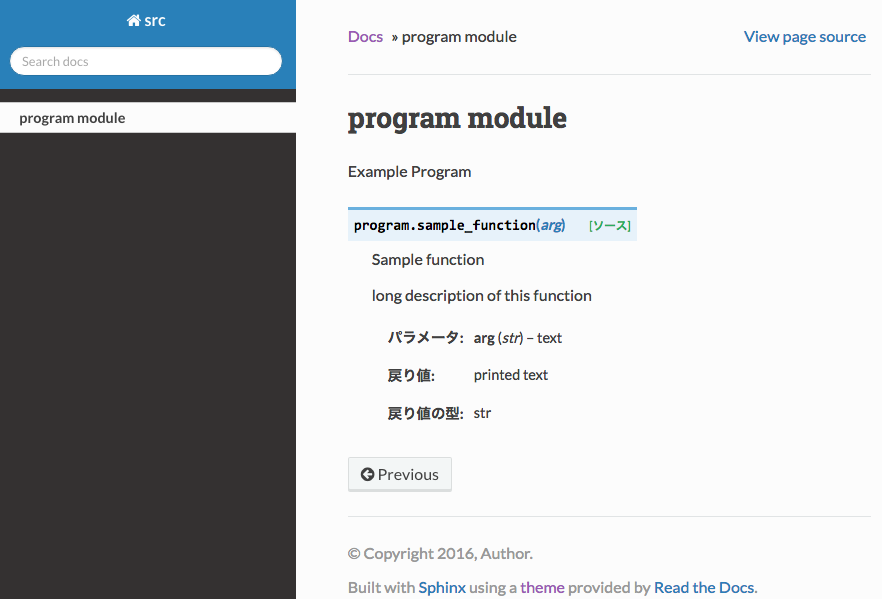
\includegraphics[width=8cm]{img/sphinx_dst.png}
    \end{figure}
\end{frame}
\begin{frame}{なぜ使うのか?}
    \begin{itemize}
        \item ドキュメントはプログラムの理解に不可欠
        \item きちんとコメントを書こう
        \item きちんと綺麗なコメントを書こう
        \item ルールに則ったコメントを書こう
    \end{itemize}
\end{frame}
\section{まとめ}
\begin{frame}
    Pythonにはライブラリがたくさん

    きちんと使って楽をしよう
\end{frame}
\begin{frame}[standout]
  Questions?
\end{frame}
\end{document}
